\documentclass{beamer}
\setbeamertemplate{caption}[numbered]

\usepackage{graphicx}

\title{Slideshow test with {\LaTeX}}
\author{yaboi}

\usetheme{Frankfurt}

\begin{document}

\maketitle

\section{Introduction}

\begin{frame}
\frametitle{Roadmap}

\begin{itemize}
\item Frames\pause
\item Beamer themes\pause
\item Pauses and slides\pause
\item Sections\pause
\item Images\pause
\item Columns
\end{itemize}

\end{frame}

\section{Data}

\begin{frame}
\frametitle{Statistics on People}

\begin{itemize}
	\item There's lots of em
	\item Deeefinitely lots of em
\end{itemize}

\begin{block}{Fact}
	I'm definitely correct
\end{block}

\end{frame}

\begin{frame}
\frametitle{More data}

I ran out of data ):

\end{frame}

\section{Images}

\begin{frame}
\frametitle{Images}

\begin{centering}
	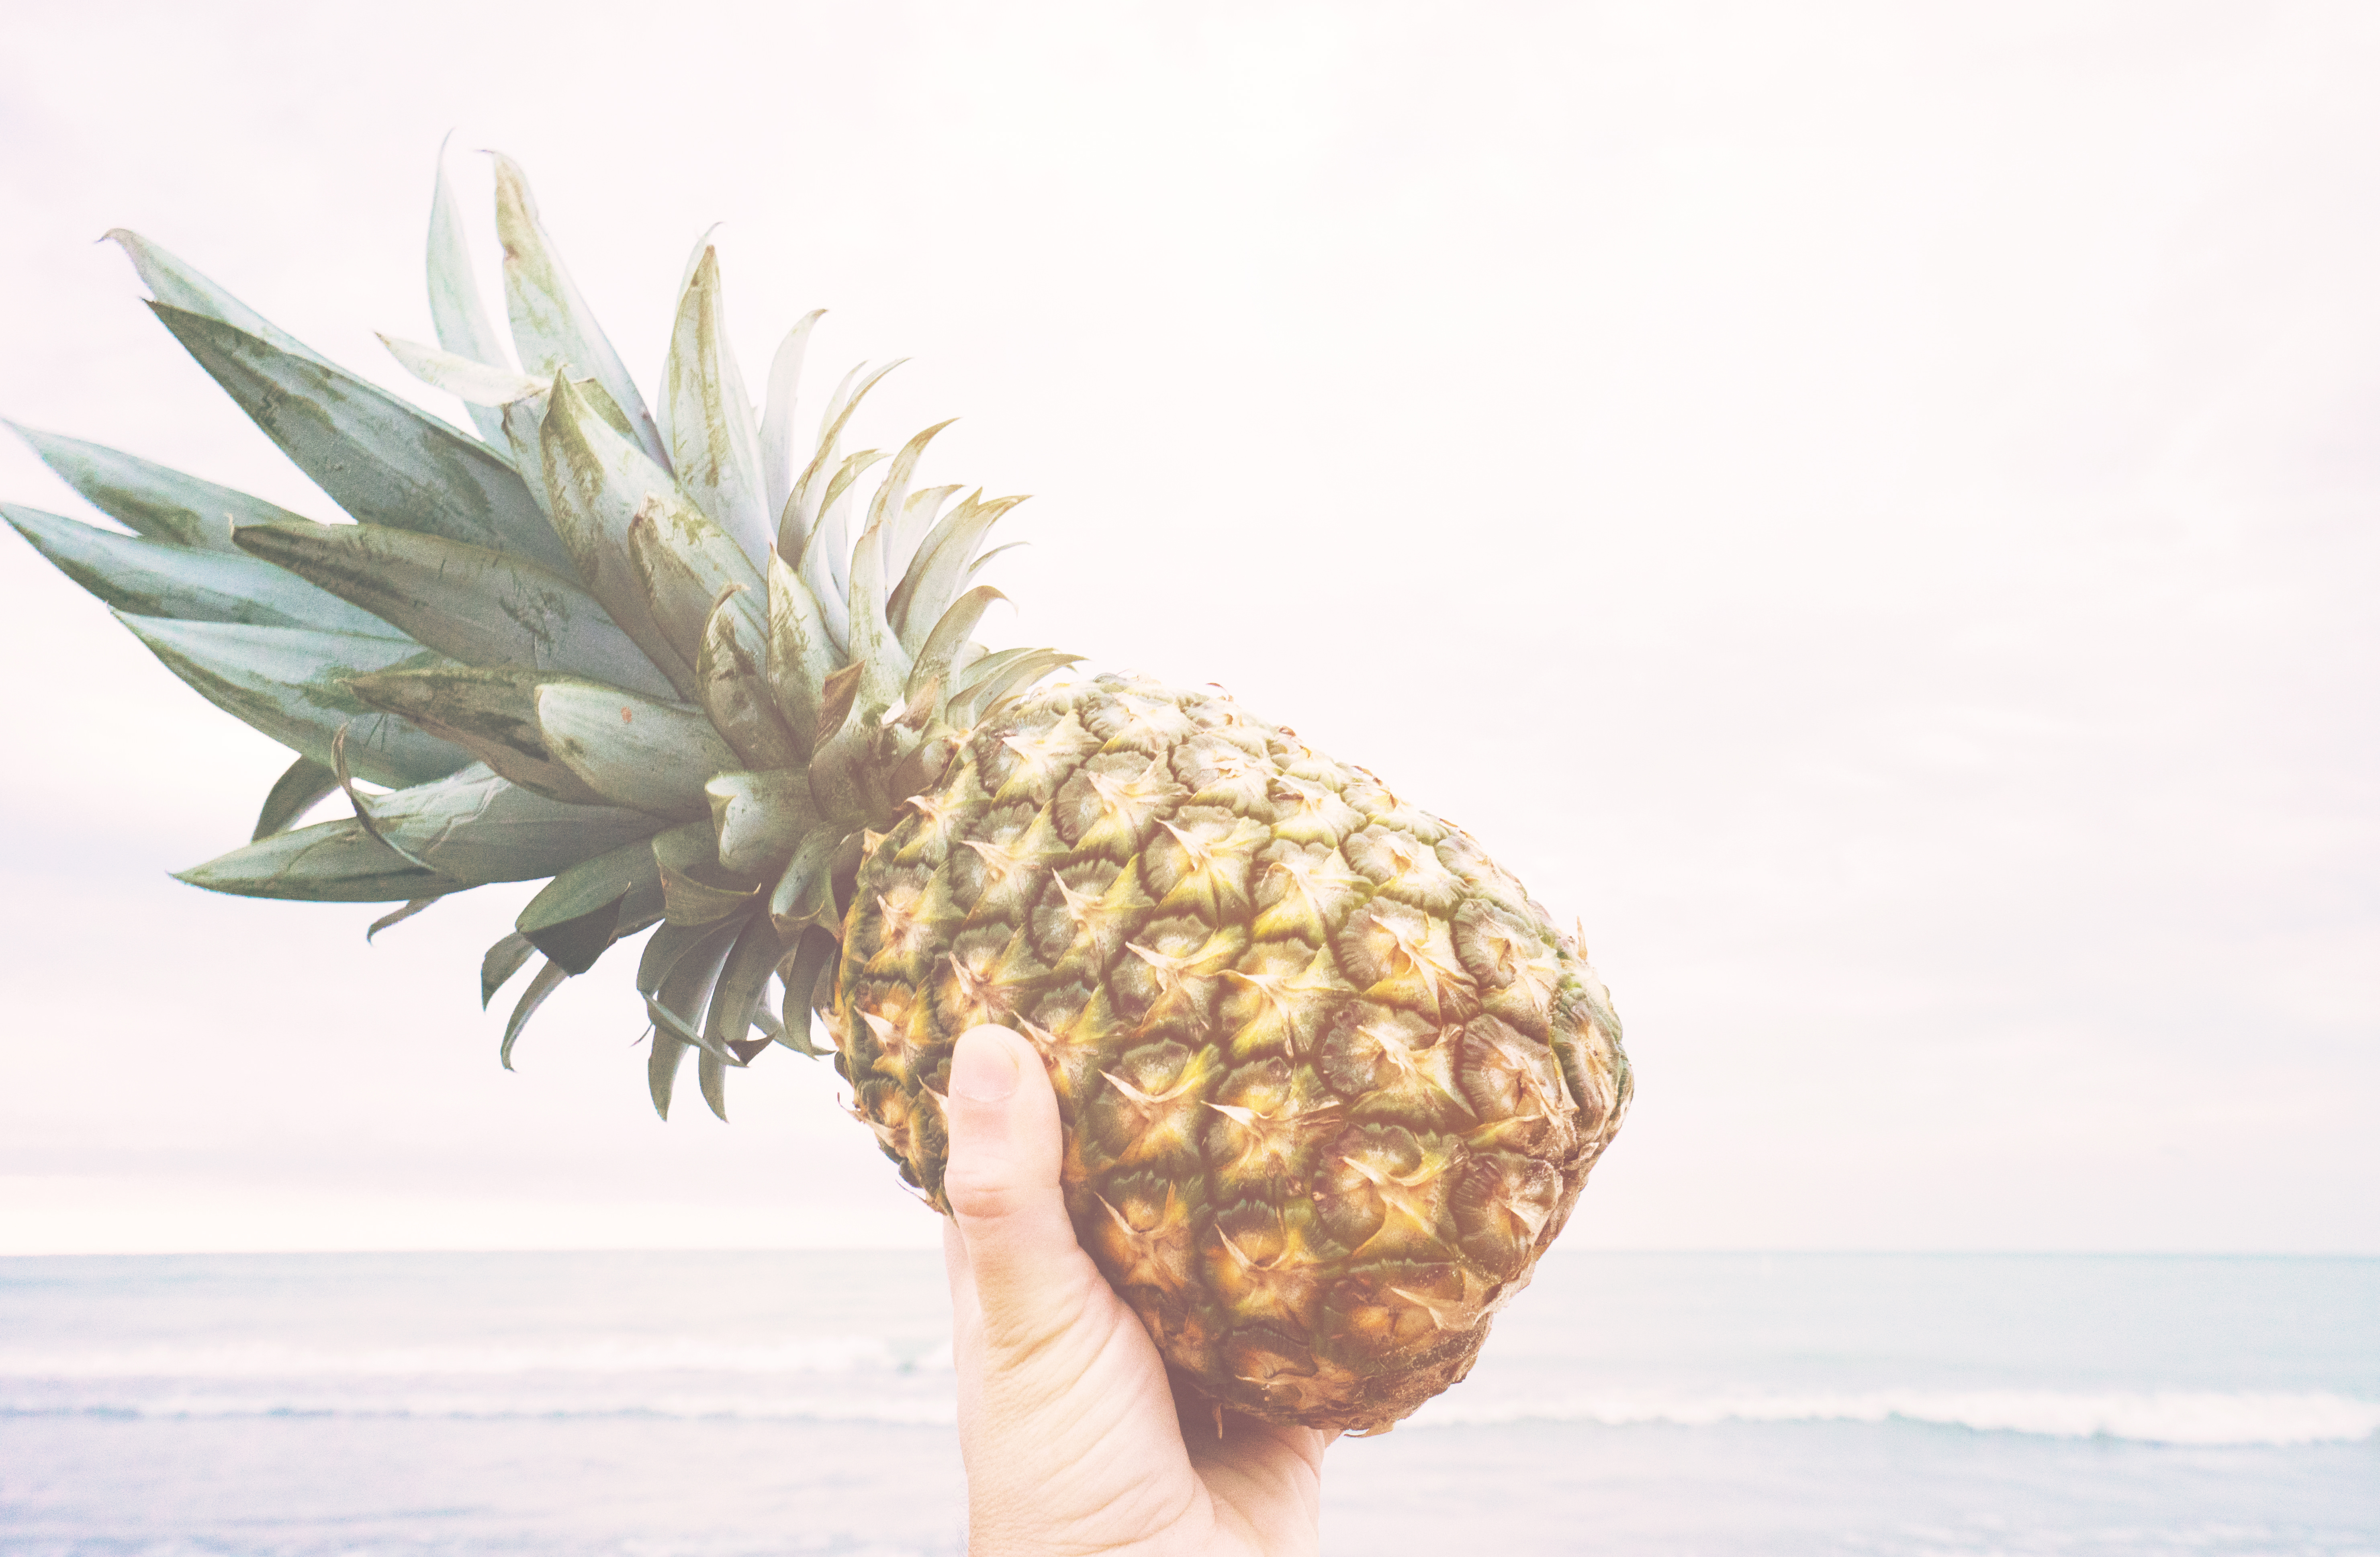
\includegraphics[height=0.85\textheight,width=0.85\textwidth,keepaspectratio]{main.jpg}
\end{centering}


\end{frame}

\section{Columns}
\begin{frame}
\frametitle{Columns}
\begin{columns}

\column{0.5\textwidth}
    On the right you will see Figure \ref{fig:clip}, it is a clip thing we made.

\column{0.5\textwidth}
    \begin{figure}
        \centering

        \includegraphics[height=0.85\textheight,width=0.85\textwidth,keepaspectratio]{clip.png}
        \caption{Picture of our design}
        \label{fig:clip}
    \end{figure}


\end{columns}
\end{frame}

\end{document}
